%!TEX root = ../../thirdYearReport.tex

Within T4.1 IIT developed in the first and the second year of the 
project a theoretical framework for estimating whole-body
dynamics from distributed multimodal sensors \cite{nori2015}. Considered sensors
include joint encoders, gyroscopes, accelerometers and force/torque sensors.
Estimated quantities are position, velocity, acceleration and (internal and
external) wrenches on all the rigid bodies composing the robot articulated
chain. In the third year of the project, IIT investigated the integration
of this estimation techniques with the classical identification techniques
for inertial parameters that were implementer in software packages as part of T1.4 .

In \cite{nori2015}, the estimation of dynamics quantities was performed by using 
the uncertancy of each sensor  was learned using real data.
In particular the Expectation-Maximization algorithm was used to estimate the covariance matrix of 
each sensor. IIT focused on extending this EM algorithm to also learn the mass,
center of mass and inertia matrix of each link of the robot.
This extension was validated in simulation and submitted in \cite{traversaro2015parametersEM}. 
 
%%%%%%%%%%%%%%%%%%%%%%%%%%%%%%%%%%%%%%%%%%%%%%%%%%%%%%%%%%%%%%%%%%%%%%%%%%%%%%%%
\subparagraph*{Whole-body human dynamics estimation for compliant human-robot interaction}
\begin{figure}
\centering
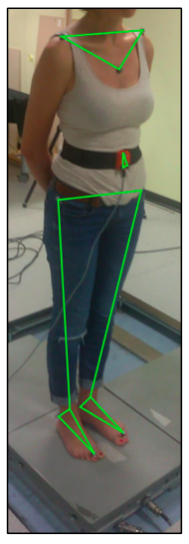
\includegraphics[scale=0.20]{images/subject.png}	\quad 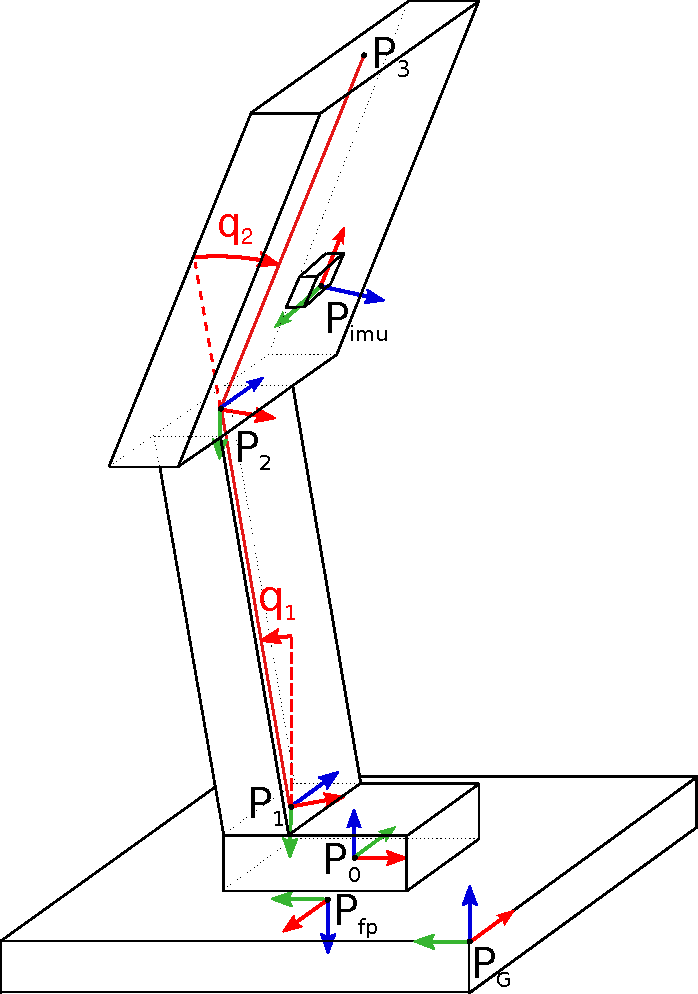
\includegraphics[scale=0.20]{images/model_refs.pdf} \quad 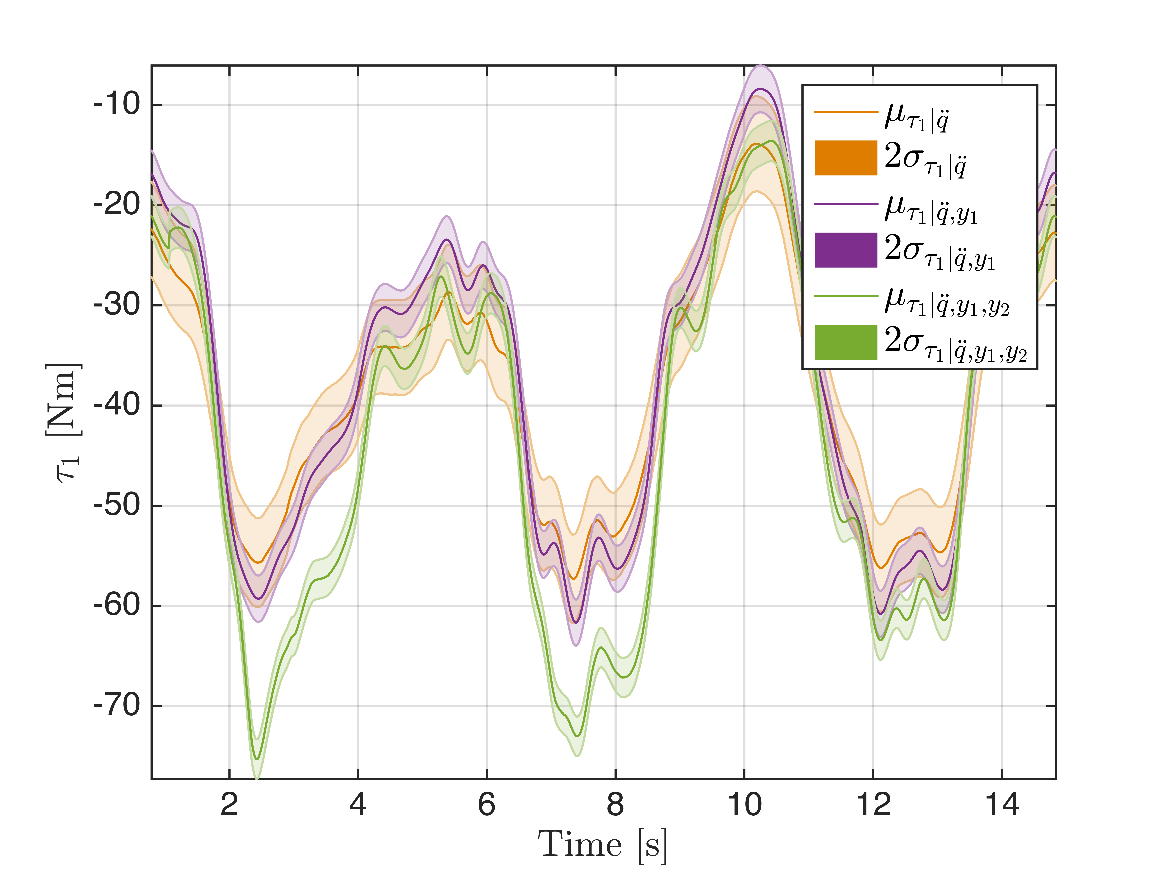
\includegraphics[scale=0.25]{images/tau1.pdf} \quad 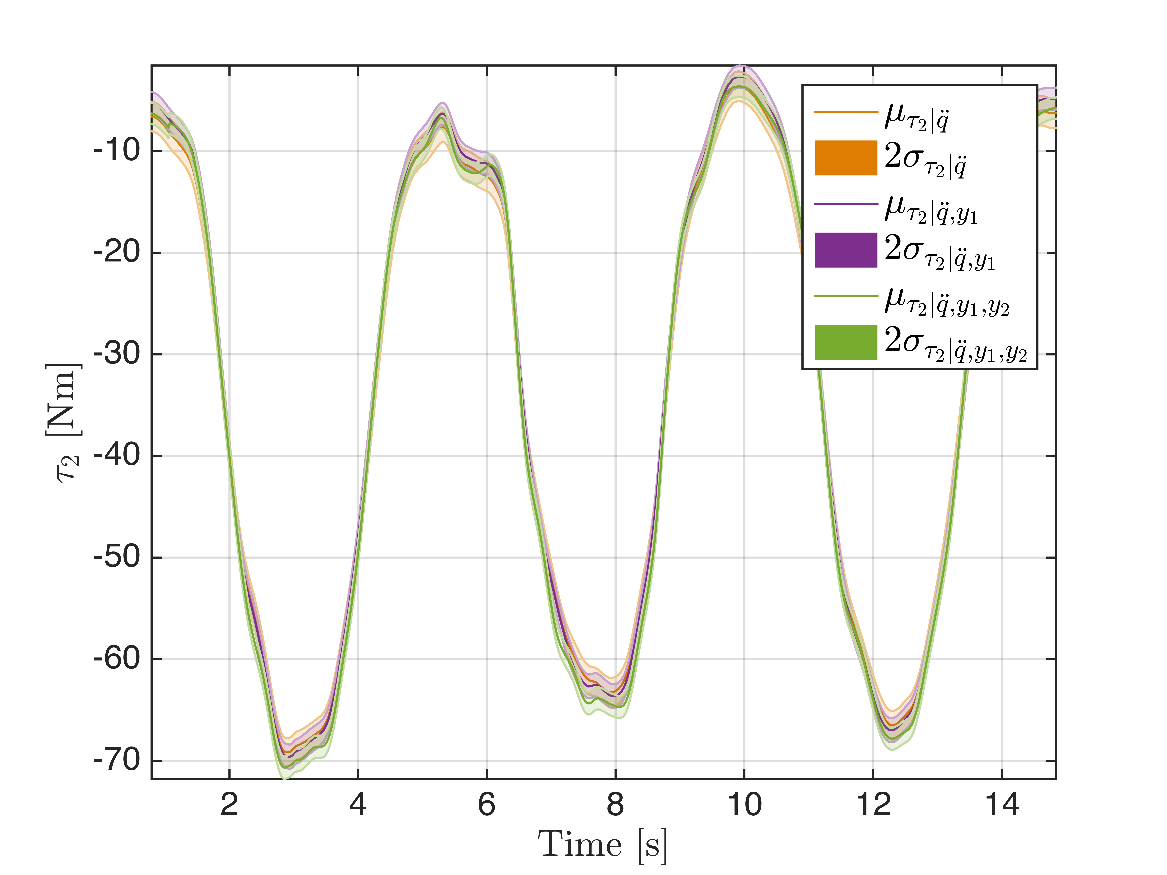
\includegraphics[scale=0.25]{images/tau2.pdf}
\caption{Perliminary experiment for real-time estimating human whole-body dynamics with distributed accelerometers and force/torque sensors. The technology is the same originally devloped for the iCub, modified to becomes a wearable technology. At present a single IMU and force-plate are used. In this preliminary experiment only ankle and hip torques were estimated.}
\end{figure}

%~\par
Although not directly scheduled as a task for the third year, IIT is currently involved in the development of a human wearable prototype of sensors suit which has strong connections with WP2 and will be a fundamental technology for the last year of the project and the associated validation scenario.  The proposed suit tracks human motions and records the forces that he is exchanging with the robot giving real-time  whole-body estimations of the human dynamics.  This novel technology will endow robots with the ability to understand and control physical collaboration in human-robot physical interaction.

\textit{Introduction and problem statement:} Human whole-body motion tracking is nowadays a well-established tool in the analysis of human movements. Well known examples include: a wearable marker-less technology suitable for outdoor motion capturing produced by Xsens \cite{roetenberg2009xsens}, a state-of-the-art marker-based technology for in lab applications produced by Vicon, and Microsoft's Kinect depth camera system which allows marker-less low-cost whole-body motion tracking for  indoor applications \cite{zhang2012microsoft}.
Although existing technologies provide a high level of accuracy in computing motion quantities, they have several limitations in measuring kinetic quantities in real-time (kinetics considers forces that cause movements).  A key problem lies in the fact that motion capture methods typically employ only kinematic measurement modalities (position, velocities and accelerations) \cite{Bonnet2013} and does not include information on the kinetics of human movements.  
Whole-body force tracking is not a new challenge for the scientific community but the topic has been seldom explored \emph{in situ} due to the computational difficulties of the analysis and even more rarely analyzed in a real-time modality. Although several recent studies are going in this direction, it is limited to prototypical and non-wearable technologies. 

\textit{ Methodology:} Our methodology attempts to estimate dynamics quantities by exploiting the fusion of the sensor information on a probabilistic Gaussian framework in presence of redundant (and noisy) measurements \cite{Latella2015}.  The framework is based on the idea of building a joint probability for all the dynamic variables and measurements coming from multiple sensors and to compute the estimation as the conditioned probability of the variables themselves given the measurements.  Preliminary results show that the variance associated to each estimated variable decreases as the number of considered measurements (sensors) increases.
